\subsection{Implementation details}
\label{subsec:noah__genesis_implementation}

I will now describe a few features of GENESIS pulse programmes, as well as how their generation is implemented in code.
GENESIS is written in TypeScript; during website deployment, this is compiled to JavaScript, which can then be directly executed in the client's web browser.
No server-side code is employed, meaning that the GENESIS web page is actually a static site; it is currently hosted using GitHub Pages.

\begin{mylisting}[!htbp] % lst:genesis_sc {{{1
\begin{tcbminted}{bruker}
/* PREAMBLE */
; gns_noah2-SCqf
; 13C HSQC
; 1H magnitude-mode COSY
"d4          = 0.25s/cnst2"  ; 13C INEPT
"in0         = inf1/2"       ; 13C HSQC increment
"in11        = 2*dw"         ; COSY increment
; ...
define delay DC_HSQCa
"DC_HSQCa    = d4-p14/2"
"l0          = td1/2"        ; TD1/NBL

/* MAIN SECTION */
1 ze
4 d1 st0
  ; MODULE 1 - HSQC
  (p1 ph0):f1
  ; ...
  goscnp ph30 cpd2:f2
  50u do:f2
  2m st
  ; MODULE 2 - COSY
  (p1 ph12):f1
  ; ...
  go=2 ph26
  1m iu1        ; TD1/NBL counter
  1m igrad EA   ; echo–antiecho gradients
  1m id11       ; COSY t1
  30m wr #0 if #0 zd
if "l1 % 2 == 0" {
  1m id0        ; HSQC t1
}
  lo to 4 times l0
exit

/* EPILOGUE */
ph0=0
;gpnam4: SMSQ10.100
;gpz4: 70% (13C CTP)
;cpd2:wvm:wudec: cawurst_d-20(220 ppm, 1.4 ms; L2H)
;d4: 1/4J(CH)
;auprog: noah_hsqc:noah_cosy QF
;module identifiers: C_HSQC H_COSY_QF
;pulse programme created by genesis-v2.2.2, https://nmr-genesis.co.uk
;Sun Sep 11 2022 16:04:54 GMT+0800 (Malaysia Time)
\end{tcbminted}
    \caption[Abridged GENESIS pulse programme]{Abridged GENESIS pulse programme for the \noah{S,C} supersequence shown in \cref{fig:noah_timings_noah_sc}.}
    \label{lst:genesis_sc}
\end{mylisting} % }}}1

\subsubsection{Overall structure}

The structure of a pulse programme can loosely be separated into three parts, which are shown in \cref{lst:genesis_sc}:
\begin{enumerate}
    \item the \textit{preamble}, which consists of everything up until the beginning of the actual pulse sequence (signified by the \texttt{ze} command). This includes header comments as well as definitions of parameters, such as delays and pulse widths;
    \item the \textit{main section}, which contains the actual pulse sequence;
    \item the \textit{epilogue}, which contains phase cycle information as well as footer comments describing each parameter. Instructions for generating shaped pulses using Bruker's WaveMaker software are also included here, as well as instructions for automatic processing (\cref{subsec:noah__genesis_processing}), and comments indicating how the pulse programme was generated (for reproducibility purposes).
\end{enumerate}

The algorithm used for pulse programme construction can be broken up into similar sections.
The construction of the preamble and main section is largely accomplished through the collation of \textit{module-specific information}, the most important of which are:
\begin{itemize}
    \item descriptive information about the modules themselves, which go into the header comments;
    \item parameter definitions, which are collated to form the preamble. Duplicates must be removed here to avoid errors; and
    \item the pulse programmes themselves, which are directly concatenated to form the main section.
\end{itemize}
These, as well as other smaller bits of information (e.g.\ relevant citations, appropriate processing scripts), are stored within \texttt{NOAHModule} objects (an example is provided in \cref{lst:module_c_hsqc}).
Each distinct module corresponds to one such object.
Therefore, if one wants to add a new module to GENESIS, most of the work can be completed by simply defining a new \texttt{NOAHModule} object: no changes to the algorithm itself are needed.

\begin{mylisting}[!ht] % lst:module_c_hsqc {{{1
\begin{tcbminted}{typescript}
let shortDescription = `; 13C HSQC`

let preamble = `
"d4      = 0.25s/cnst2"                ; 13C INEPT
; ...
"D[ID]a  = d4-p14/2"
`   // [ID] is later replaced with the module code

let pulprog = `
  ; 13C-1H HSQC

  ; INEPT
  (p1 ph0):f1
  ; ...
  goscnp ph30 cpd2:f2
  50u do:f2
`

const mod = new NOAHModule(
    "C_HSQC",           // internal module code
    "c13",              // module category
    "S",                // single-letter code, Table 4.1
    [],                 // relevant citations (if any)
    "noah_hsqc",        // AU programme for processing
    shortDescription,   // short description
    [AF_EDIT],          // available acquisition flags
    preamble,           // preamble text
    pulprog,            // pulse programme text
    1,                  // number of FIDs
    false               // flag for 'parallel' modules
);
export default mod;
\end{tcbminted}
\caption[HSQC \texttt{NOAHModule} object]{An excerpt of the \texttt{NOAHModule} object for the HSQC module shown in \cref{fig:noah_sb_po_s} (internal code \texttt{C\_HSQC}).}
    \label{lst:module_c_hsqc}
\end{mylisting} % }}}1

To put the epilogue together, the pulse programme constructed so far is scanned for pulse phases, shaped pulses, and all other parameters.
Using predefined lookup tables, GENESIS then creates pulse phase definitions, WaveMaker directives (where appropriate), and comments containing textual descriptions of each parameter.
These comments are not merely cosmetic; they are also displayed in the \texttt{ased} screen when setting up an experiment.
Finally, instructions for automatic processing of the NOAH data (to be explained in \cref{subsec:noah__genesis_processing}) are added to the bottom, together with a timestamp and the version number of GENESIS for reproducibility purposes.

\subsubsection{Phase/delay incrementation and looping}

Since NOAH experiments are 2D experiments, there is one additional complication: the pulse programme must contain appropriate looping statements, together with pulse phase and delay incrementation, in order to correctly generate the indirect dimension.
In many existing NOAH pulse programmes, looping in 2D experiments was written using the equivalent of nested \texttt{for} loops (\cref{lst:genesis_looping}, \textit{left}).
Although this structure suffices for the vast majority of supersequences, whenever any parameter must be incremented in a different manner (e.g.\ in parallel supersequences where multiple supersequences are interleaved, or when using the PSYCHE module which has a different number of $t_1$ increments), the nested loop structure must be modified, which is not easy to reason about.
I therefore opted to change the structure to use only one loop, and to control the phase and delay incrementation using modular arithmetic (\cref{lst:genesis_looping}, \textit{right}).
The outcome is entirely equivalent, but this strategy allows for other cases to be implemented simply by adding another check on the loop counter \texttt{L1}.

\begin{mylisting}[!ht] % lst:genesis_looping {{{1
\begin{tcbmintedsbs}{bruker}
\begin{minted}[fontsize=\small]{bruker}
"l0 = td1/4"


1 ze
3 1m
4 d1 st0

  ; ... (pulse sequence goes here)

  ; in inner loop
  1m igrad EA   ; HSQC gradients
  1m id11       ; COSY t1
  30m wr #0 if #0 zd
  lo to 4 times 2

  ; in outer loop
  1m ip5*2      ; HSQC 13C 90
  1m ip30*2     ; HSQC receiver
  1m id0        ; HSQC t1
  lo to 3 times l0



end
\end{minted}
\tcblower
\begin{minted}[fontsize=\small]{bruker}
"l0 = td1/2"
"l1 = 0"

1 ze
4 d1 st0


  ; ... (pulse sequence goes here)

  ; on every pass
  1m iu1        ; loop counter
  1m igrad EA   ; HSQC gradients
  1m id11       ; COSY t1
  30m wr #0 if #0 zd

  ; on every second pass
  if "l1 % 2 == 0" {
    1m ip5*2      ; HSQC 13C 90
    1m ip30*2     ; HSQC receiver
    1m id0        ; HSQC t1
  }
  lo to 4 times l0

end
\end{minted}
\end{tcbmintedsbs}
    \caption[GENESIS implementation of looping]{Implementation of phase/delay incrementation and looping in previous NOAH sequences (\textit{left}, using nested loops) and in GENESIS (\textit{right}, using modular arithmetic).}
    \label{lst:genesis_looping}
\end{mylisting} % }}}1


\subsubsection{Parameter standardisation}

Each NOAH module contains a number of parameters, including pulse widths, delays, gradient amplitudes, and shaped pulse waveforms.
Since different modules are stored separately (as different \texttt{NOAHModule} objects), directly concatenating their pulse programmes may lead to conflicting parameter definitions if appropriate care is not taken.
GENESIS avoids this by maintaining a global table of parameter definitions which are applicable to all modules: when new modules are added, they must be checked against this to ensure that there are no inconsistencies.

In general, where possible, these parameters are chosen to be consistent with pulse programmes in the Bruker standard library: thus, for example, \texttt{P1} is the \proton{} \ang{90} pulse width, and \texttt{CNST2} is the $\oneJ{CH}$ value used for calculating INEPT (and other) delays.
This makes it easy to read in parameters either from the \textit{prosol} (probe and solvent) relation tables in TopSpin, or from other existing parameter sets.
Some delays are module-specific and do not need to be reused, and in standard library sequences, are often labelled as \texttt{DELTA1}, \texttt{DELTA2}, and so on.
To avoid conflicting definitions and also to improve readability, I renamed these such that they include the name of the module: thus, in a \carbon{} HSQC these may be labelled \texttt{DC\_HSQC\_1}.
Here, \texttt{C\_HSQC} is the name associated with the \texttt{NOAHModule} object.

If combined with some caution when adding new modules, these measures ensure that there will be no parameter clashes between the modules \textit{within a given supersequence}: we may view this as a \textit{local uniqueness} of parameters.
However, the impact of this design choice is even more far-reaching:
since parameters are stored globally, they will always have the same value in \textit{all possible supersequences} (or in other words, the parameters are \textit{globally unique}).
Thus, \texttt{CNST2} in a \noah{B,S} supersequence has the same meaning as \texttt{CNST2} in a \noah{B,S,C} supersequence (and so on).
This makes it exceptionally easy to set up multiple different supersequences in TopSpin using GENESIS pulse programmes, as virtually all of the parameter values may simply be copied from a previous NOAH dataset.

One potential issue with this strategy is that TopSpin provides only a finite number of named pulse widths (for example).
Thus, there are only so many different parameters which can be stored in a global table before running into inevitable conflicts.
A workaround would be to sacrifice the global uniqueness of each parameter, and only have it be unique within a given supersequence.
Fortunately, this situation has not (yet) surfaced.%
\footnote{The number of \textit{pulse phases} in GENESIS is in fact dangerously close to the maximum number of 32. However, the global uniqueness criterion is not really important for pulse phases, because---unlike, say, delays---pulse phases are hardcoded in the pulse programme, and cannot be copied from one dataset to another. So, if necessary, I could dispense with the global uniqueness for pulse phases only, at the cost of some increased code complexity. I did briefly contemplate this possibility, but since I am at the end of my DPhil and am unlikely to add any new modules soon, this will likely remain a hypothetical.}


\subsubsection{Parameter descriptions}

At the epilogue of the pulse programme, extra comments are added for every parameter present in the pulse programme.
Most of these are purely textual in nature, and appear in the TopSpin \texttt{ased} parameter setup screen; this naturally helps to make the pulse programmes as easy to use as possible.
However, some of these comments have special meanings: gradient amplitudes and shapes, for example, are specified in a way which allows them to be automatically populated using the \texttt{gppp} Python script packaged with TopSpin.
Furthermore, WaveMaker directives are also specified for some shaped pulses, allowing them to be created in an on-the-fly manner using the \texttt{wvm} command.
This means that the user (generally) need not separately download and install a set of shaped pulses.

\subsubsection{Module choice}

One final issue which must be overcome is the fact that some NOAH modules may be implemented differently depending on the supersequence which it is being used in.
The HMBC module described in \cref{subsec:noah__case_studies} is one such example: the form of the $zz$-filter depends on whether the HMBC module is required to retain \magn{C} and/or \magn{N} magnetisation for subsequent modules.
Thus, in the \noah{B,S} supersequence the $zz$-HMBC must be used, but in the \noah{S,B} supersequence the `original' HMBC without a $zz$-filter is preferable.
Since these have different pulse programmes, each of these `versions' of the HMBC are described by \textit{separate} \texttt{NOAHModule} objects (\texttt{C\_HMBC\_CF} and \texttt{C\_HMBC\_NOF} respectively).

However, it is unlikely that the majority of users would want to manually configure the supersequence in such detail by selecting \texttt{NOAHModule} objects.
Thus, the GENESIS web interface actually hides these different versions from the user, only showing one button labelled `HMBC'.
Under the hood, the logic above is used to deduce the correct version of the HMBC based on what other modules the user has chosen (\cref{fig:hmbc_flowchart}).

\begin{figure}[htb]
    \centering
    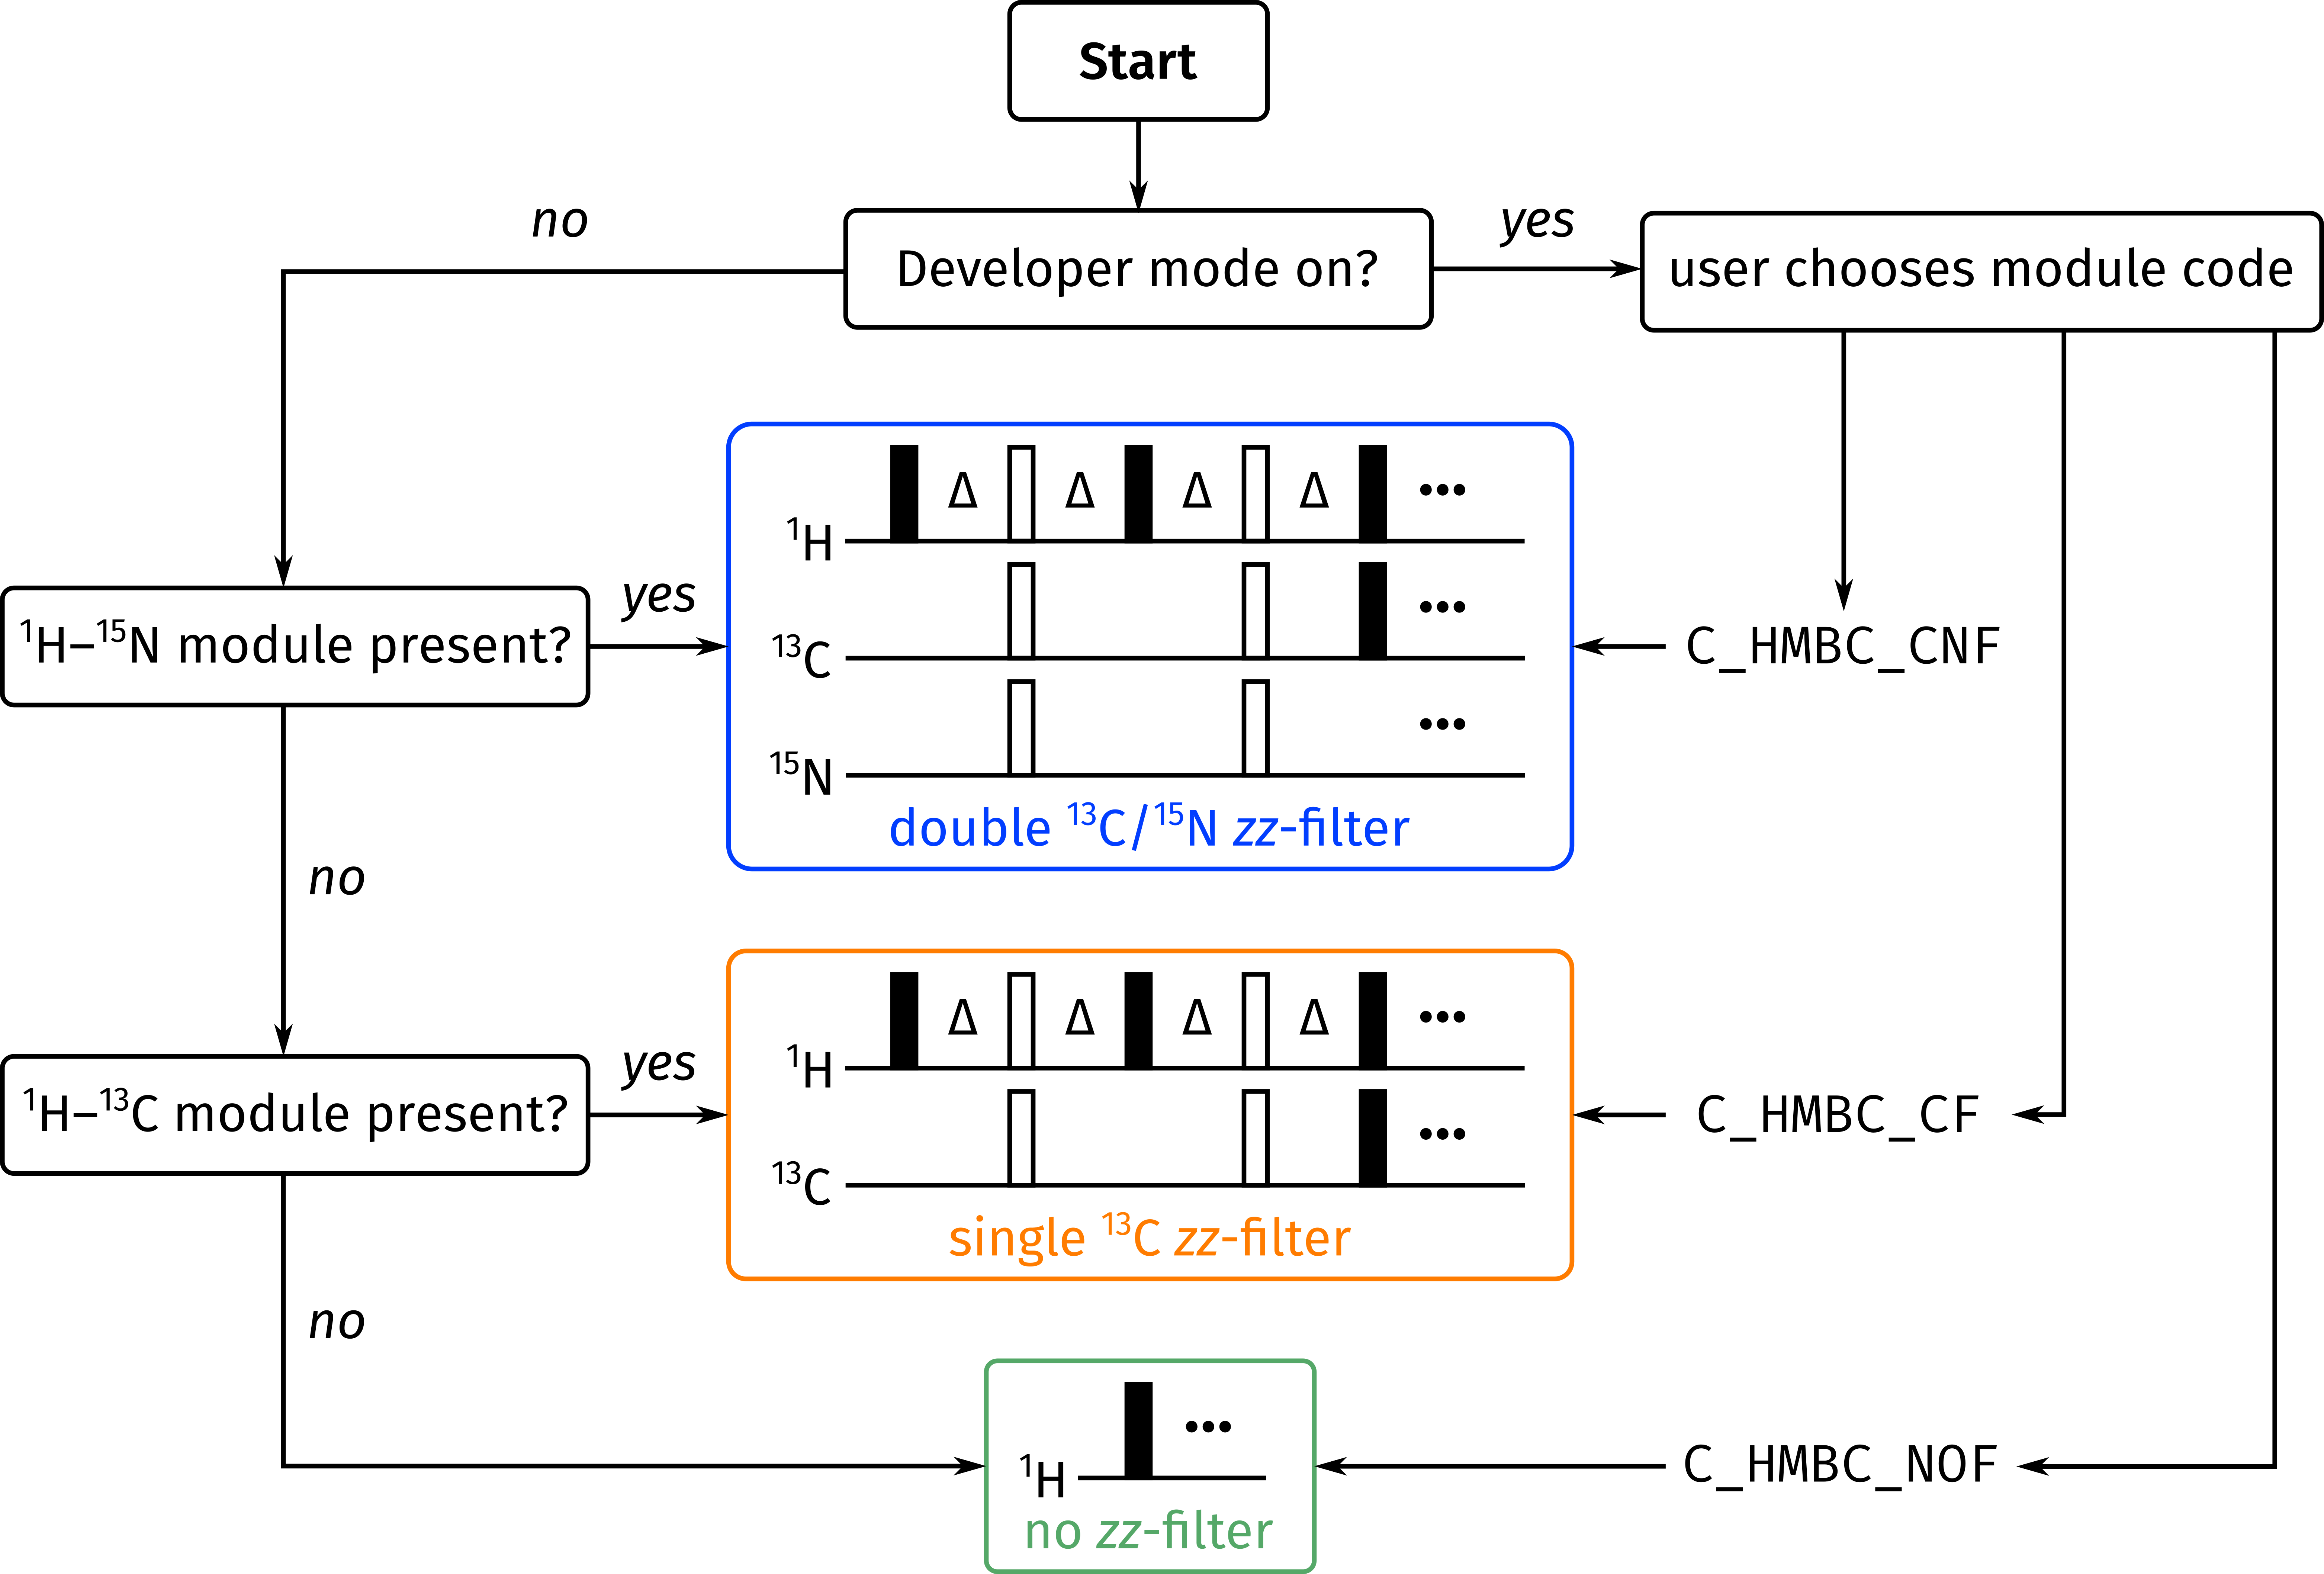
\includegraphics[]{noah/hmbc_flowchart.png}%
    \caption[Flowchart for choosing HMBC module version]{
        Flowchart showing how the correct `version' of the HMBC module is determined when constructing a supersequence using GENESIS.
        When developer mode is on, the user directly chooses module codes corresponding to each version of the HMBC.
        When it is off, the appropriate version is chosen based on which other modules are present in the supersequence.
    }
    \label{fig:hmbc_flowchart}
\end{figure}

Should the user indeed want to control the exact module used, the website also offers a `developer mode' switch: turning this on allows the user to directly choose the desired module.
(Enabling developer mode also reveals a handful of extra modules which were used exclusively for my DPhil and are not generally of interest.)


\subsubsection{Tests}

One risk inherent in any NMR experiment is the possibility of causing spectrometer damage when executing malformed pulse programmes.
To minimise the chances of this, each version of GENESIS is checked against a series of automatic tests before being released.
The most important tests ensure that every module containing decoupling statements also turns off decoupling immediately after acquisition.
On top of this, there are also a series of regression tests where (some representative) supersequences are checked against the same ones produced by previous versions of GENESIS: any differences in these are automatically flagged for review.
The live website is only updated if all tests are passed.

However, none of this can actually \textit{stop} GENESIS from creating wrong pulse programmes.
For example, if a module with an incorrect pulse programme is created, then any supersequence containing that module will not be fully functional.
There is no adequate way to check for this, as GENESIS cannot verify the correctness of an NMR experiment.
However, the inclusion of the tests described above minimises the chances of creating pulse programmes which are outright dangerous; any mistakes will at worst lead to the wrong (or no) data being obtained.
It should be mentioned that this is not a \textit{new} problem which GENESIS introduces: errors in pulse programmes can arise equally easily (if not \textit{even more easily}) when they are handwritten.


\subsubsection{Reproducibility}

The final section of a GENESIS pulse programme consists of comments intended solely for reproducibility purposes.
These comments indicate exactly which \texttt{NOAHModule} objects were used to create the pulse programme, as well as a GENESIS \textit{version number}.
Since GENESIS has been updated with some regularity during my DPhil, each release is assigned a version number, which broadly follows the principles of \textit{semantic versioning}.
Old versions of GENESIS may be accessed by navigating to the specific URL \texttt{https://nmr-genesis.co.uk/X/Y/Z} for version \texttt{X.Y.Z}.
Then, after enabling developer mode, the specific list of \texttt{NOAHModule} objects may be input in order to create the corresponding pulse programme.
Thus, these two pieces of information together allow all GENESIS pulse programmes to be exactly regenerated whenever necessary: this is important in ensuring that the data thus acquired are reproducible.


\subsubsection{How smart is GENESIS?}

Having written several pages of text about the \textit{features} present in GENESIS, it is tempting to think that it is `intelligent' in its design of pulse programmes.
I have, at various points in time, received suggestions for extensions to the concept: in GENESIS, the building blocks used for pulse programme construction are NOAH modules, but one could envision breaking up these into the smallest possible units of pulses, delays, gradients, and so on, and using something like GENESIS to construct \textit{arbitrary} pulse programmes.
This was even speculatively mentioned in the GENESIS paper\autocite{Yong2022AC}.

However, in truth, GENESIS is a long way from being able to do such things.
In particular, it does not have any actual understanding of the Bruker pulse programming syntax: \textit{almost} all of the pulse programme instructions are hardcoded as strings.%
\footnote{There are several exceptions where some parameters (for example, loop counters in DIPSI mixing) are dynamically generated, mainly to avoid clashes between different parts of the supersequence.}
Thus, the creation of pulse programmes is not \textit{truly} being done from the ground up: instead of `combining pulse sequence elements', a more accurate description is that the \textit{text} corresponding to different pulse sequence elements is being concatenated.
There is actually a substantial amount of brute force involved, and this is also why it is not possible for the automated tests to really check the correctness of the pulse programmes.

Of course, it is hardly a trivial task to write something more sophisticated: I would need to construct abstract representations of each pulse sequence element (pulses, delays, etc.), and functions which could translate these into actual pulse programme commands.
I feel that I would need rather more knowledge in computer science, especially a course on compilers.
However, this was something I would have very much liked to do had I had more time!
I will also leave open the possibility of---although I do not \textit{commit to}---expanding the GENESIS code in this direction as a future personal project.
